\section{付録とは}
付録とは本や雑誌などについてくるおまけのようなもののことである.

\subsection{サブセクション}
サブセクションも使えると考えれる。


\newpage
\section{画像}
画像(がぞう)は、2次元平面上に描かれた絵を指す。
画像には静止画(静止画像)と動画(動画像)とがあるが
動画像は映像と呼ばれることが多く、この項目では静止画像について記述する。
コンピュータ上の静止画像はデジタルカメラの写真や、コンピュータグラフィックスなどから生成されたものがあり、自動的、半自動的な画像処理や画像認識に向くという特徴がある。

\begin{figure}[htbp]
\begin{center}
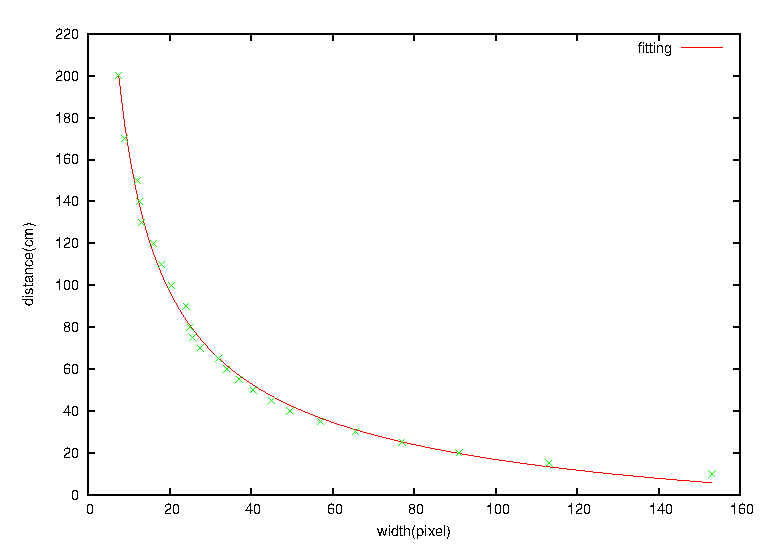
\includegraphics[width=0.5\linewidth]{appendix/eps/pixy.eps}
\caption{XXXXの画像}
\label{ラベルの名前}
\end{center}
\end{figure}

\newpage

\section{表}
表は、ビジュアルコミュニケーションの一形態であり、データを並べる手段である。
テーブルはコミュニケーション、研究、データ解析など様々な分野で使われている。
印刷物、手書きのノート、コンピュータソフトウェア、建築装飾、交通標識など様々なところでテーブルを見つけることができる。
\begin{table}[htbp]
\caption{XXXXの表}
\begin{center}
\begin{tabular}{|cl|}
\hline
主翼幅 & 880[mm] \\
主翼面積 & 1325[cm$^2$] \\
平均翼弦& 150[mm] \\
水平尾翼面積 & 267[cm$^2$] \\
モーメントアーム長 & 500[mm] \\
水平尾翼容積 & 0.67[-] \\
重心位置 & 75[mm] \\
         & (平均翼弦の50\%) \\
機長 & 840[mm] \\
機体重量 & 470[g] \\
(バッテリー含む) &  \\
\hline
\end{tabular}
\end{center}
\end{table}

\newpage

\section{fverbatimの例}
fverbatimをfigureで囲むことで図として扱っている.

\begin{figure}[htbp]
\begin{fverbatim}{1.1\linewidth}
◎ [armadillo300 ~]# fdisk /dev/hda
hda: hda1
◎ Command (m for help): d
Selected partition 1
◎ Command (m for help): n
Command action
   e extended
   p primary partition (1-4)
◎ p
\end{fverbatim}
\caption{コマンド手順1}
\label{ラベル名}
\end{figure}
